\documentclass[tikz,border=6pt]{standalone}
\usepackage{amsmath,amssymb}
\usepackage{xcolor}
\definecolor{accent}{HTML}{A13D2C}
\definecolor{accent2}{HTML}{2B5F6B}
\definecolor{muted}{HTML}{5A564F}
\definecolor{panel}{HTML}{F8F6F0}
\definecolor{linecol}{HTML}{D8D2C4}
\definecolor{astroblue}{HTML}{1B4F72}
\usetikzlibrary{calc,arrows.meta}
\begin{document}
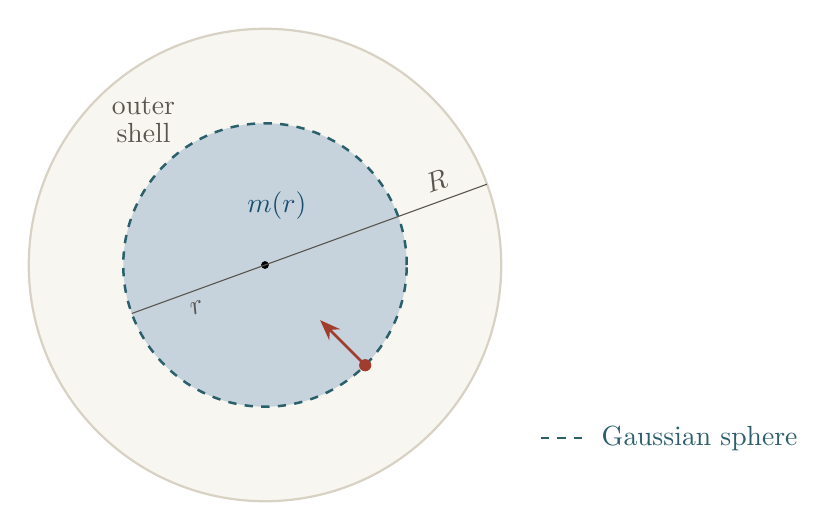
\begin{tikzpicture}[scale=1.0, >={Stealth[length=2.6mm]}]
  % star of radius R = 3, inner ball of radius r = 1.8
  \def\R{3.0}\def\r{1.8}
  \fill[panel] (0,0) circle (\R);
  \draw[linecol, line width=0.8pt] (0,0) circle (\R);
  \fill[astroblue!25] (0,0) circle (\r);
  \draw[accent2, dashed, line width=0.9pt] (0,0) circle (\r);
  \fill (0,0) circle (1.4pt);
  % radius lines (labels beside the line, never on an arrow)
  \draw[muted] (0,0) -- ({\R*cos(20)},{\R*sin(20)});
  \node[muted, above, rotate=20] at ({0.80*\R*cos(20)+0.0},{0.80*\R*sin(20)+0.02}) {$R$};
  \draw[muted] (0,0) -- ({\r*cos(200)},{\r*sin(200)});
  \node[muted, below, rotate=20] at ({0.55*\r*cos(200)},{0.55*\r*sin(200)-0.02}) {$r$};
  % labels of the two regions
  \node[astroblue] at (0.15,0.75) {$m(r)$};
  \node[muted, align=center] at ({0.5*(\R+\r)*cos(130)},{0.5*(\R+\r)*sin(130)}) {outer\\[-2pt]shell};
  % a parcel on the Gaussian sphere and the pull it feels, toward the centre
  \coordinate (P) at ({\r*cos(-45)},{\r*sin(-45)});
  \fill[accent] (P) circle (2.2pt);
  \draw[->, accent, line width=1.0pt] (P) -- ($(P)!0.45!(0,0)$);
  % legend for the dashed circle, placed outside the star
  \draw[accent2, dashed, line width=0.9pt] (\R+0.5,-2.2) -- (\R+1.1,-2.2);
  \node[right, accent2] at (\R+1.15,-2.2) {Gaussian sphere};
\end{tikzpicture}
\end{document}
